\documentclass[11pt]{article}
\title{Assignment 6: Latex G5}
\author{Group 5: Alexandros Tsiridis, Stamatis Maritsas, Andray Afanasyev}
\date{}
\usepackage{url}
\usepackage{graphicx} 
\usepackage{placeins}
\usepackage{listings}
\usepackage{color}
\addtolength{\oddsidemargin}{-.875in}
\addtolength{\evensidemargin}{-.875in}
\addtolength{\textwidth}{1.75in}
\addtolength{\topmargin}{-.875in}
\addtolength{\textheight}{1.75in}
\begin{document}
\maketitle
\tableofcontents
\listoffigures
\listoftables

\section{XML - XPointer}
\subsection{Introduction}
XPointer is a system that allows the creation of links that point to components of XML. It is divided among four specifications:
\begin{enumerate}
\item XPointer framework
\item XPointer element() scheme
\item XPointer xmlns() scheme
\item XPointer xpointer() scheme
\end{enumerate}
The above points are going to be explained further to the subsections below. It is worth mentioning that XPointer Framework is a W3C recommendation since March 2003.

\subsection{XPointer framework}

The XPointer framework's specification defines the XML Pointer Language (XPointer), which is an extensible system for XML addressing and includes the XPointer schemes that mentioned in the introduction.

This framework can be used as a specification for creating XML fragment identifiers for resources whose media type is one of text/xml, application/xml, text/xml-external-parsed-entity, or application/xml-external-parsed-entity. In addition, it is also encouraged to use this framework to define your own fragment identifier language. \cite{xpointerframework}

\subsection{XPointer element() scheme}

This kind of XPointer scheme is tend to be used to allow basic addressing of XML elements. Furthermore, the formal grammar for this scheme is given using simple EBNF (Extented Backus-Naur) notation as described in the XML Recommendation.\cite{elementscheme}

\subsection{XPointer xmlns() scheme}

The purpose of this scheme is to interpret the namespace prefixes in pointers correctly. For example, a developer can create his own namespaces and place them in an XML document and then use the xmlns() scheme to point to those namespaces. Just like the XPointer element() scheme, the formal grammar for the xmlns() scheme is given using simple EBNF notation, as described in the XML Recommendation.\cite{xmlnsscheme} 

\subsection{XPointer xpointer() scheme}

The role of this scheme in the whole XML XPointer philosophy is to address efficiently fragments of XML documents. In order to achieve this goal it uses the XPath and adds the ability to address strings, points and ranges. It supports addressing not only into the internal structures of XML documents but also to external parsed entities. Moreover, it allows the examination of a document's hierarchical structure and choice of portions based on various properties (i.e. element types, etc.). Another thing that I have to mention is the fact that, the xpointer() scheme's extensions to XPath provide the ability to identify locations that are not single, whole elements and combine string matching with the other location methods supplied.\cite{xpointerscheme}

\subsection{XML XPointer in practice}

There are two ways of linking a part of an XML document:
\begin{itemize}
\item We can simply add a number sign (\#) and an XPointer expression after the URL in the xlink:href attribute, as follows:
\textcolor{cyan}{\textit{xlink:href="http://dog.com/dogbreeds.xml\#xpointer(id('Rottweiler'))"}}. The expression refers to the element in the target document, with the id value of \underline{"Rottweiler"}.
\item XPointer also allows a shorthand method for linking to an element with an id. You can use the value of the id directly, like this: \textcolor{cyan}{\textit{xlink:href="http://dog.com/dogbreeds.xml\#Rottweiler"}}.
\end{itemize}
\begin{figure}[!htb]
\centering
  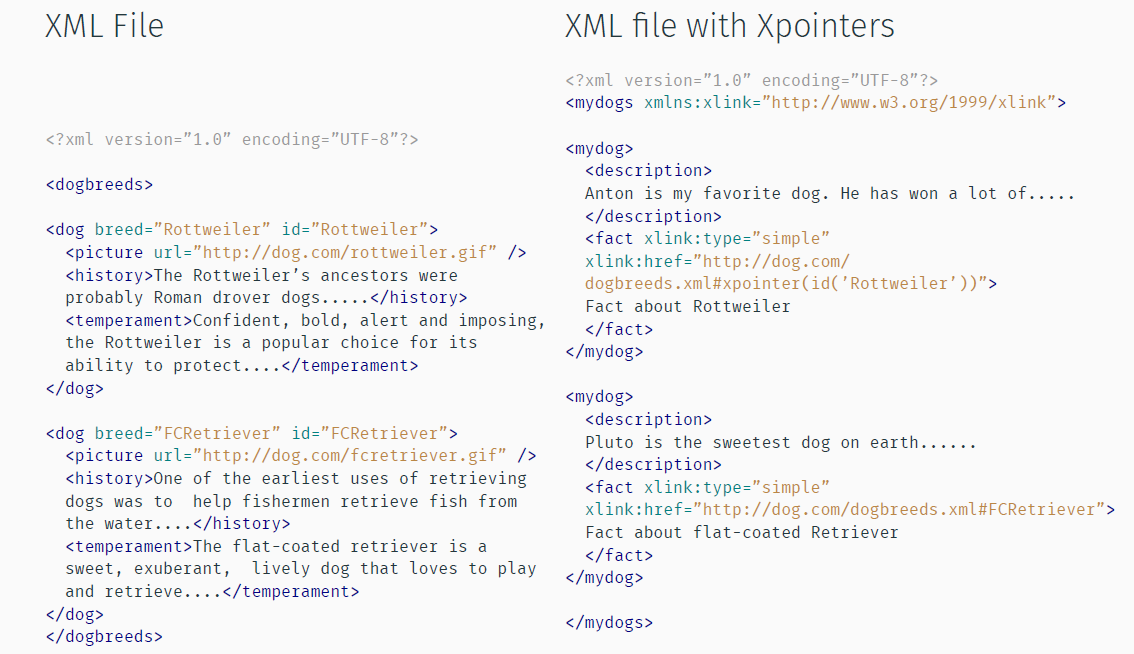
\includegraphics[width=.9\linewidth]{images/xpointerExample}
  \caption{Example code of the two ways (modified version) \cite{W3CSchools}}
  \label{fig:xpointerExample}
\end{figure}
\FloatBarrier

\subsection{XPointer VS XPath}

\begin{table}[!htb]
\centering
 \begin{tabular}{||c || c||} 
 \hline
 \textbf{XPointer} & \textbf{XPath}\\ [0.5ex] 
 \hline
 same expression & same expression\\ 
 \hline
 specifies the connections of URIs & says nothing about URIs \\
 \hline
 new features introduced & no available features \\
 \hline
\end{tabular}
\caption{Comparison of XPointer and XPath}
\label{table:xpointerVSxpath}
\end{table}
\FloatBarrier

\section{Overhauling Amd for the ’00s: A Case Study of GNU Autotools}

\subsection{Introduction}

As group 5 we were assigned to look at the above article and discuss it during the lecture. In the following section, I am going to discuss about the article and what information I believe is useful to grasp from the paper, and what I learned from it. First of all, I will break up the article in three parts:
\begin{enumerate}
\item \underline{How the build was done before the \textbf{autotools} and what autotools have to offer}.
\item \underline{Measuring complexity}.
\item \underline{What you can gain by the use of \textbf{autotools}}.
\end{enumerate}

\subsection{How the build was done before the autotools and what autotools have to offer}

Without the use of \textbf{autotools}, the building and configuration of the package is being done manually by the user and the programmer of it. At the first step, users have to manually configure a package before the compilation by changing the header file. In order to achieve this goal, the user need to have intimate knowledge of the system that he was trying to install the package on.

Moreover, in order for the programmers to achieve desired compatibility for the packages they are making use of extended \textcolor{red}{CPP macros}. These macros are being used to recognize features that the operating system need to have due to them being dependencies of the package. Such macros are complicated to write and usually end up in an extended nested form. Due to the complexity of the macros and their nested forms, maintenance of the package by the programmers becomes a nightmare.

Another way that is being used is the Imake utility which is designed specifically for building X11 applications. This tool defines static configurations for various systems, which cannot be account for local changes made by the user. One more utility which is being used is Metaconfig. This utility executes simple tests to find out the features of the system, but needs a lot of interaction with the user to confirm that the detection is correct.

\textbf{GNU autotools} were created in order to address the problems that were mentioned above. This is achieved by providing in build tests to dynamically detect various features of the system that are needed for the package. It is a suite of three tools namely \textit{Autoconf, Automake and Libtool}.

\subsection{Measuring complexity}
In this subsection I am going to talk about three ways of measuring complexity that were mentioned in the article. I find these information quite useful even if someone is not interested in \textbf{autotools} or how to build a package without the use of them. In the paper, the three ways of measurement are:
\begin{itemize}
\item \underline{Measuring complexity according to the amount of the code lines inside the package}.
\item \underline{Measuring complexity according to the amount of total \textcolor{red}{CPP macros} across the whole package}.
\item \underline{Measuring complexity according to the average of total \textcolor{red}{CPP macros} per 1000 lines of code}.
\end{itemize}

The first measurement will obviously make the biggest package the most complex. In my opinion, this is not an accurate way of measuring complexity as a bigger package might actually be less complex than a smaller one.

\begin{figure}[!htb]
\centering
  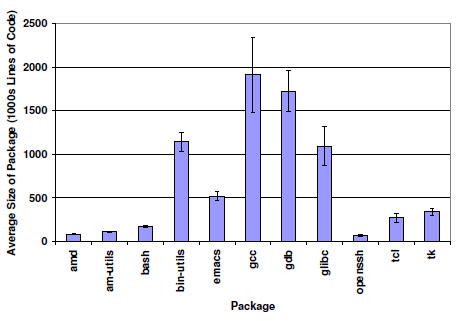
\includegraphics[width=.7\linewidth]{images/measure1}
  \caption{Average size of packages in thousands of lines of
code \cite{zadok2002}}
  \label{fig:measure1}
\end{figure}
\FloatBarrier
The second measurement its a bit more accurate than the way discussed above. It also has a fault as bigger packages usually tend to have more \textcolor{red}{CPP} conditionals than the smaller ones making them candidates for being the most complex ones in this measurement.

\begin{figure}[!htb]
\centering
  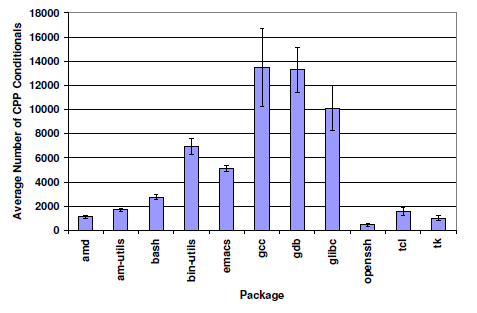
\includegraphics[width=.7\linewidth]{images/measure2}
  \caption{Average number of \textcolor{red}{CPP} conditionals per package \cite{zadok2002}}
  \label{fig:measure2}
\end{figure}
\FloatBarrier

The third measurement in my opinion, is better than the above two as it actually counts how often \textcolor{red}{CPP} commands are introduced inside the code.

\begin{figure}[!htb]
\centering
  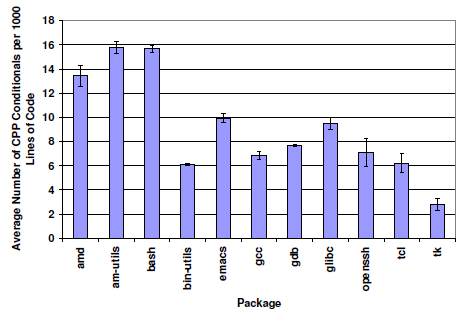
\includegraphics[width=.7\linewidth]{images/measure3}
  \caption{Average number of \textcolor{red}{CPP} conditionals per 1000 lines
of code \cite{zadok2002}}
  \label{fig:measure3}
\end{figure}
\FloatBarrier
To sum up, let's take the packages example seeing in the figures of \textcolor{green}{gcc} and \textcolor{blue}{amd}. In the first figure, \textcolor{green}{gcc} climbs to the top of the complexity scale as the biggest package and \textcolor{blue}{amd} is second from last due to its small size. In the second measurement, \textcolor{green}{gcc} is also the most complex one by a small difference from \textcolor{cyan}{gdb} and \textcolor{blue}{amd} is third from last. And at the last measurement, where the size of the package does not actually matter, \textcolor{green}{gcc} is fourth in complexity from last and \textcolor{blue}{amd} climbs to the third most complex package.

\subsection{What you can gain by the use of autotools}
By the use of \textbf{autotools} there are various benefits as well as a few disadvantages that are introduced. First of all, they reduce the complexity of code by automating the feature discovery procedure. They minimize the use of \textcolor{red}{CPP} conditionals by providing those in build tests. On the other hand, they do not reduce to zero the usage of those macros as they do not cover all the possible tests that the package might need to do. BY the reduction of complexity, as shown in the article, programmers become more rapid developers as they introduce more features in less time than they did without the use of \textbf{autotools}. In addition, the programs are easier to maintain by the developers and easier to be installed by the users as the process of building and compiling the package becomes automated.

On the other side of the coin, \textbf{autotools} are not perfect and they have their disadvantages. Firstly, the developers need  to be well-trained and used to these tools. This procedure, of learning the tools, takes a significant amount of time as stated at the article, it took them 54 months to learn how to use \textbf{autotools} properly. Secondly, \textbf{autotools} are making the compilation significantly slower as stated in the article, it took three times more time to compile their package with \textbf{autotools} than the version that did not use \textbf{autotools}. \textit{The result of the test performed on the article can be seen at the following table:}

\begin{table}[!htb]
\centering

\begin{tabular}{|l|r|}
\hline
Action and Package & Time\\ \hline
Build Amd-upl102 & 35.4\\ \hline
Configure Am-utils-6.0a1 (no cache) & 102.6\\
Configure Am-utils-6.0a1 (with cache) & 24.2\\
Compile Am-utils-6.0a1 & 73.1\\ \hline
\end{tabular}
\caption{Time (seconds) to Configure and Build Amd Packages \cite{zadok2002}}
\label{table:buildTest}
\end{table}
\FloatBarrier

In my opinion, \textbf{autotools} are useful to be learned by companies that produce a lot of software as the process of learning the \textbf{autotools} will provide them with less complex programs in the future. In addition, companies that provide long term packages will also be benefit by using those tools.

\nocite{*}
\bibliographystyle{plain}
\bibliography{bibliography}

\end{document}